\documentclass{article}
\usepackage{graphicx, amsmath, amssymb, multirow}
\usepackage{geometry} 
\geometry{
  a4paper,
  total={170mm,257mm},
  left=20mm,
  top=20mm,
}

\begin{document}

\section{Image Tests}

Inline image: 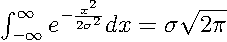
\includegraphics[width=0.15\textwidth]{test.png}

\begin{figure}[h]
    \centering
    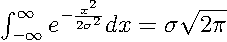
\includegraphics[width=0.7\textwidth]{test.png}
    \caption{Test image centered in a figure environment.}
    \label{fig:test_image}
\end{figure}

\newpage

\section{Some beautiful mathematical equations}

Ramanujan's formula:

$$\frac{1}{\pi}=\frac{2\sqrt{2}}{9801}\sum_{k=0}^\infty\frac{(4k)! (1103+26390k)}{(k!)^4 396^{4k}}$$

Euler's formula: $e^{i\pi}+1=0$

Area of triangle with sides a,b,c is: 

$$A=\frac{1}{2} \sqrt{s(s-a)(s-b)(s-c)},\quad s=\frac{a+b+c}{2}$$

The most important formula in calculus:

\[
  f'(x)=\lim_{h\to 0}\frac{f(x+h)-f(x)}{h}
\]

Einstain's field equations:

\[
R_{\mu\nu}-\frac{1}{2}g_{\mu\nu}R+\Lambda g_{\mu\nu}=\frac{8\pi G}{c^4}T_{\mu\nu}
\]

Gamma function:

\[
  \Gamma(z) = \int_0^\infty t^{z-1} e^{-t} dt,\quad\Gamma(z+1) = z \Gamma(z)
\]

Pythagora's theorem:

$$a^2+b^2=c^2$$

Logarithms: 

$$\log ab=\log a+\log b$$

Navier-Stokes equation:

$$\rho\left(\frac{\partial \textbf{v}}{\partial t}+\textbf{v}\cdot\nabla\textbf{v}\right)+\nabla p=\nabla\cdot\textbf{T}+\textbf{f}$$

Law of gravity:

$$F=G\frac{m_1m_2}{r^2}$$

Fourier transform:

\[
  F(\omega) = \int_{-\infty}^\infty f(t) e^{-2\pi i t \omega} dt
\]

Maxwell's equations: 

\begin{equation}
\nabla \times \textbf{E}=\frac{\rho}{\epsilon_0}
\end{equation}

\begin{equation}
\nabla \cdot \textbf{H}=0
\end{equation}

\begin{equation}
\nabla \times \textbf{E}=-\frac 1c\frac{\partial \textbf{H}}{\partial t}
\end{equation}

\begin{equation}
\nabla \times \textbf{H}=\frac 1c\frac{\partial \textbf{E}}{\partial t}
\end{equation}

Schroedinger equation:

\[
i \hbar \frac{\partial \psi}{\partial t} = H\Psi
\]

Chaos theory:

$$x_{t+1}=kx_t(1-x_t)$$

Information theory:

\[
  H=-\sum p(x)\log p(x)
\]

Black-Scholes equation:

$$\frac12\sigma^2S^2\frac{\partial^2V}{\partial S^2}+rS\frac{\partial V}{\partial S}+\frac{\partial V}{\partial t}-rV=0$$

Second law or thermodynamics:

$$dS\ge 0$$

Mass-energy equivalence:

$$E=mc^2$$

Basel problem:
\[
  \frac{\pi^2}{6}=\sum_{n=1}^\infty \frac{1}{n^2}
\]

Euler-Masceroni constant:

\[
\gamma = \lim_{n\to\infty}(\sum_{n=1}^\infty \frac{1}{n}-\log n)\approx 0.5772156649\ldots
\]

Binomial expansion:

\[
  (a+b)^n = \sum_{k=0}^n \binom{n}{k} a^k b^{n-k}  
\]

Gauss:

$$\int_{-\infty}^\infty e^{-x^2} dx = \sqrt{\pi}$$

The Callan-Symanzik equation:

\[
\left[M\frac{\partial}{\partial M}+\beta(g)\frac{\partial}{\partial g}+n\gamma\right]G^n(x_1,x_2,...,x_n;M,g)=0
\]

Minimal surface equation:

$$\mathcal{A}(u)=\int_\Omega(1+|\nabla u|^2)^{1/2} dx_1 dx_2 ... dx_n$$ 

Multiline equations:

\begin{eqnarray*}
\cos{2\theta} & = & \cos^2\theta - \sin^2\theta \\
              & = & 2\cos^2\theta - 1 \\
              & = & 1 - 2\sin^2\theta
\end{eqnarray*}

And finally:

$$1=0.999999999999999999\ldots$$

Just for fun: $6 + 9 + 6 \cdot 9 = 69$

\end{document}
